% Included after the empirical overview. These are selected independently
% verified examples, not additional population-level empirical tables.
\section{Independent finite-radius verification of trained networks}
\label{sec:verified-trained-networks}
The aggregate empirical audits above use numerical sufficient inequalities and numerical attacks.  This section separates out selected positive and negative examples checked by exact rational arithmetic and outward interval evaluation.  A certificate for all real inputs is distinguished from an exhaustive certificate on a specified finite Boolean domain.  Both quantify over every allowed disturbance.  A pointwise certificate covers every disturbance at one specified input, while a negative witness is one verified input--disturbance pair.  These scopes are kept distinct.

\paragraph{Global certificates for raw trained models.}
The global restriction is satisfied by some ordinary, unconstrained trained networks.  A width-256, depth-4 tanh network trained by minibatch SGD on all 60,000 MNIST images for even-versus-odd classification has test accuracy $98.94\%$, no training errors, and minimum signed training output exceeding $2.6876$.  Its raw saved weights satisfy the global condition at $c=.003$: for every real input and every allowed simultaneous disturbance, the raw output changes by at most $0.032296<1/16$.  This global bound was verified using exact rational operator-norm certificates and a rational final gain comparison, rather than relying on a floating-point spectral estimate.

There are also eligible depth-16, width-128 examples at $c=.001$: the selected SGD models for continuous and thresholded-Boolean MNIST 3-versus-8 inputs have minimum training margins exceeding $.6918$ and $4.236$, respectively, test accuracy $99.29\%$ and $99.19\%$, and rigorously verified global raw-change bounds $.060795$ and $.062230$.  These use raw trained weights, without output rescaling.  Their global certificates apply to every real input, so imply either clipped-score convention.  The radius constant matters: for the latter Boolean model we independently verified violations at $c=.01$ on both a held-out image and a Boolean cube probe, with clipped-score changes exceeding $.08450$ and $.08553$, respectively.  The successful small-radius certificate and larger-radius failure are compatible.

\paragraph{An exploratory inverse-depth calibration.}
A later, separate calibration sets $c_H=.001/H$.  For the depth-16 full-MNIST model \texttt{105}, which has a verified global failure at the original $c=.001$, exact rational spectral bounds prove global raw-output variation at most $.02365730<1/16$ at $c_H=1/16000$.  Thus this same trained parameterization passes a weaker, explicitly depth-dependent support condition.  This is not a revision of the original protocol or evidence that a fixed $c$ works uniformly in depth.  Since the theoretical bound has polynomial dependence on $c+c^{-1}$, such a polynomial depth calibration preserves a polynomial formal sample bound.  The training-eligible depth-$32$ continuation \texttt{301} also has an exact global raw-change bound $.01782087$ at $c_H=1/32000$, despite its verified failure at fixed $c=.001$.

\paragraph{Projected SGD at a larger fixed radius.}
All four predeclared projected-SGD models (depths $4$ and $16$, width $256$, on full MNIST parity and Fashion-MNIST shirt-versus-T-shirt) have exact rational certificates that every internal matrix has operator norm below one.  Their global raw-output change bounds at $c=1/16$ are respectively $.061573$, $.058087$, $.061573$, and $.058087$, all below $1/16$.  The corresponding test accuracies are $98.95\%$, $98.87\%$, $87.10\%$, and $86.20\%$.  None attains every training margin above $1/2$: this is evidence that the support condition can coexist with useful trained prediction, not an example satisfying the paper's exact interpolation likelihood.
The separately declared longer-training continuation \texttt{600} retains an exact global bound $.058087$ at the same radius, but still has $154$ training errors after $240$ additional epochs, with $98.83\%$ test accuracy.  Thus all five projected parameterizations have verified global stability, and none is presented as satisfying the exact training-likelihood event.

\paragraph{Exhaustive Boolean-domain certificates.}
A separate, predeclared cohort trains width-$64$ tanh networks on $400$ of the $512$ vertices of $\{-1,1\}^9$, with the remaining $112$ vertices held out.  For the protocol-selected depth-$4$ majority network \texttt{500}, exact arithmetic and outward intervals certify the clipped-score condition on \emph{every} Boolean input at $c=.03$.  All $400$ training margins are independently interval-verified above $1/2$, and the network correctly predicts all $512$ labels.  The global raw-change bound is $.162903>1/16$, whereas every clean absolute output exceeds $4.72037$.  Consequently the clipped score is exactly constant under every permitted disturbance at every vertex.  A separate auditor replayed the saved matrix factors, all $512$ interval trajectories, and all $400$ training inequalities.

A subsequent, separately recorded check gives the same exhaustive conclusion for the depth-$16$ majority network \texttt{501} at the largest primary radius $c=1/16$.  Its raw-change bound is $3.474718$, while every clean absolute output exceeds $5.12034$; all $512$ labels and every training margin are correct.  These finite-domain certificates use the elementary implication
\[
 |z(x)|\ge m,\qquad |z^\eta(x)-z(x)|\le B\le m-\tfrac12
 \quad\Longrightarrow\quad
 \operatorname{clip}_{1/2}(z^\eta(x))=\operatorname{clip}_{1/2}(z(x)).
\]
They therefore certify the actual clipped-score condition even when the stronger raw-output-change condition is not certified.  Their scope is the entire finite Boolean domain, not all real inputs.

\paragraph{A depth-$64$ example requiring reachable-state bounds.}
The first depth-$64$ majority network, \texttt{504}, also satisfies the condition on \emph{all} $512$ Boolean vertices at the primary $c=.001$.  Every one of the $400$ training margins is interval-verified above $7.61170$, and every clean absolute output on the full cube exceeds $5.64786$.  Thus this network also satisfies the original all-input clean-margin restriction, not only the newer clipped-score restriction.  Exact interval label comparisons give $511/512$ correct predictions on the full cube, including $111/112$ held-out predictions; the remaining vertex is a confidently wrong prediction, not an omitted or ambiguous case.  Its global raw-change bound, $13.414533$, cannot establish this conclusion, even with output clipping.  Instead, $52$ finite groups of vertices share rigorously bounded reachable-state tubes.  Each group's disturbed outputs remain beyond the corresponding clipping threshold, with the smallest verified surplus exceeding $1.40770$.  Thus the clipped score is exactly invariant for every allowed disturbance at every vertex.  This is an exhaustive finite-domain certificate for an ordinary SGD-trained depth-$64$ network, rather than a sampled-input audit or a claim about every real input.

For completeness, sharing a tube across finitely many inputs does not alter the underlying proof.  At each layer and coordinate, replace the clean preactivation's distance from zero by the minimum of that distance over all vertices in the group.  A common prefix-energy bound then encloses every group's noisy trajectory, so the same derivative and matrix-norm bounds apply to each vertex.  The grouping only reduces computation.  Every input is still checked, and any unresolved input would prevent a full-domain conclusion.  The certificate uses exact integer matrix arithmetic, outward interval $\tanh$, saved norm-factor proposals, and explicit source hashes; it is not a Lean proof.  A separate auditor regenerated all $512$ clean interval trajectories, checked all $52$ groups and $3{,}216$ saved matrix bounds, and replayed every training inequality.  The three worst groups were additionally checked with the original pure-integer matrix-norm verifier.

\paragraph{A depth-$64$ nonlinear target.}
The corresponding recursive-majority network \texttt{505}, trained on majority of three disjoint three-bit majorities, also satisfies the clipped-score condition on the entire $512$-vertex cube at $c=.001$.  Every one of its $400$ training margins is interval-verified above $7.47388$, and every clean absolute output exceeds $2.40649$, so the original all-input clean-margin condition holds as well.  Its full-domain accuracy is $504/512$; the held-out accuracy is $104/112$.  All eight errors remain in the verified domain.

For this network, the shared reachable-tube proof establishes $511$ of the $512$ cases.  The remaining vertex, index $325$, is explicitly retained as unresolved in that component certificate.  A separate finite-radius proof propagates the exact clean-response covariance and bounds the nonlinear Taylor remainder in state norm.  It encloses the noisy output at this same vertex in $[-2.586691,-2.226290]$, proving that its clipped score is also invariant.  The composite certificate records the union of these two proofs, with model, radius, source, and component hashes; the input domain never changes.  The exceptional-vertex proof was independently replayed, including all $126$ exact matrix-norm bounds.  A further independent replay regenerated all $512$ clean trajectories, all $122$ groups and $7{,}585$ local matrix bounds, and every training margin, then checked the composite coverage.  The state-covariance inequality used for this refinement is given below.

\subsection{The global condition can fail on valid finite-grid inputs}
\label{sec:finite-grid-counterexamples}
A universal prior-support restriction and a statement about typical data are different claims.  The distinction persists after clipping at the training margin, even for a network that fits all training examples with substantial margin.  Our strongest example is an ordinary minibatch-SGD tanh network of hidden depth 16 and width 256, trained on all 60,000 MNIST images for even-versus-odd classification.  It has $98.92\%$ empirical test accuracy, and a separate exact computation verifies every signed training output above $4.4815762$.  The finite-radius counterexample below is independently verified.  The saved weights are used without rescaling.

The left image in Figure~\ref{fig:finite-grid-counterexamples} is a valid $28\times28$ eight-bit grayscale input.  At the smallest tested radius constant $c=10^{-3}$, its clean and disturbed real outputs are enclosed around
\[
 -0.00162845134\longmapsto-0.15496440197.
\]
The resulting score change exceeds $0.15333>1/16$ after clipping at either $1/2$ or $1$.  The image has a black two-pixel border, mean ink $0.17200$, and $64.2\%$ black pixels.  It is a synthetic off-data image, not an image to which we assign a natural digit label.  Its pixel $p_j$ is interpreted as the exact rational input $x_j=2p_j/255-1$; we also independently checked the same witness under the original float32 pixel preprocessing used for training.

The disturbance budget was checked using exact integer-rational arithmetic, and the two network evaluations used 100-decimal outward interval arithmetic with the saved dyadic weights.  In particular,
\[
 (1+H E_v)\left(N^{-1}\sum_{s=1}^{H}\|\eta_s\|_2^2+\xi^2\right)
 <10^{-6}.
\]
The intervals verify that every perturbed hidden coordinate remains in $[-1,1]$: their absolute values are all below $0.061110$.  Thus requiring disturbances to leave activations within their original range does not remove this counterexample.  Its scalar output disturbance has absolute value below $7.3\times10^{-10}$.  Removing it decreases the noise budget and changes either clipped score by at most that amount, so hidden disturbances alone still give a violation.  These are finite-radius witnesses, rather than conclusions drawn only from a large Jacobian or from an unverified optimization output.  They trust the interval-arithmetic implementation and are not Lean formalizations.

The right image provides a second example in a depth-32, width-128 SGD model for MNIST 3 versus 8, with test accuracy $99.09\%$.  Its output changes from $-0.0034068096$ to $-0.3168576499$ at the same $c=10^{-3}$, a clipped-score change greater than $0.31345$.  All perturbed hidden coordinates have absolute value below $0.128211$.  This second model has three training errors, so it is evidence about the naturalness of a support restriction rather than an additional example in the exact training-likelihood event.  A related near-gray eight-bit witness for this model has score change greater than $0.30799$.  The low-ink examples exclude an explanation specific to a uniformly gray background, while remaining clearly off-data.

Each exploratory search had a fixed budget declared before that search.  For the low-ink examples we solved an ink-minimizing linear program, subject to zero first preactivations and a black border, generated 4,096 stochastic roundings to the pixel grid using a fixed seed, and attacked the 16 candidates with smallest absolute clean output.  We then verified selected witnesses independently.  This protocol proves existence, not the prevalence of instability under the data distribution.  In separate probes preserving empirical one-pixel foreground probabilities and on interpolations of opposite-class test images, some violations were verified at $c=10^{-2}$; failure to find violations at smaller radii was not treated as a certificate.

\begin{figure}[t]
\centering
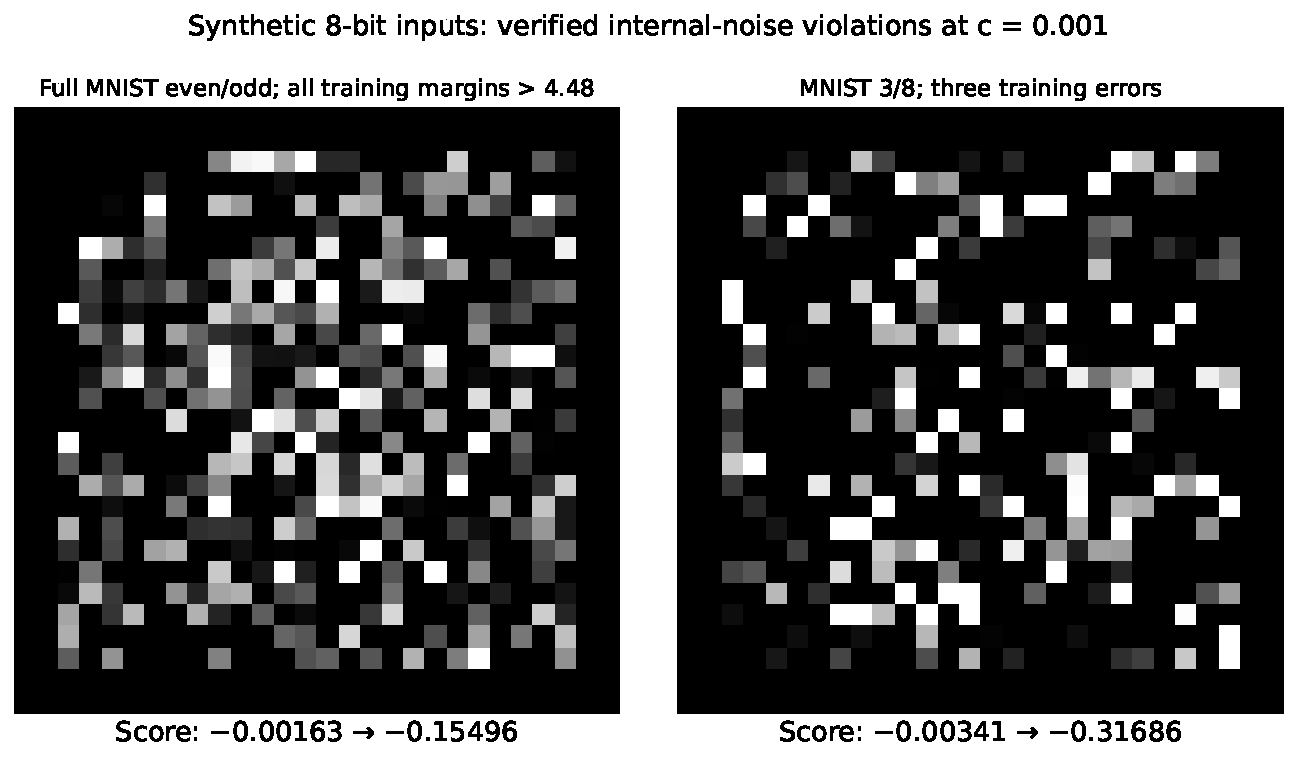
\includegraphics[width=.98\linewidth]{certificates/finite-grid-counterexamples.pdf}
\caption{Synthetic, valid eight-bit inputs violating the global clipped-score condition at $c=.001$.  Both have a fixed black border and low total ink.  The left network was trained on the full MNIST even-versus-odd task and has exactly verified training margins above $4.4815762$; the right network was trained on digits 3 and 8.  The images themselves are unchanged by the internal disturbances.  These are off-data counterexamples, not mislabeled examples from a test set.}
\label{fig:finite-grid-counterexamples}
\end{figure}

\paragraph{A precise Boolean interpretation.}
The finite-grid issue is not inherently a continuous-input phenomenon.  Write each pixel in bits $p_j=\sum_{b=0}^7 2^b q_{jb}$, with $s_{jb}=2q_{jb}-1\in\{-1,1\}$.  Since $\sum_b2^b=255$,
\[
 \frac{2p_j}{255}-1=\sum_{b=0}^7\frac{2^b}{255}s_{jb}.
\]
Replacing row $j$ of the first-layer matrix by eight rows $(2^b/255)W_{0,j}$ gives a network on $8\cdot784=6272$ Boolean inputs with exactly the same outputs, hidden trajectories, readout energy, and internal-noise budgets.  Its depth and width are unchanged.  Thus every rational-pixel witness is also an exact Boolean-input witness for this linearly decoded network.  With the usual dimension-weighted first-layer Frobenius energy, the non-bias weight contribution grows only by
\[
 8\sum_{b=0}^7(2^b/255)^2
 =\frac{8(4^8-1)}{3\cdot255^2}<2.69.
\]
The first-layer bias is unchanged but its dimension weight grows eightfold.  Consequently total first-layer energy, including the bias, increases by at most a factor of eight.
This equivalence uses exact rational pixel normalization.  The software used to train and evaluate the original model normalizes pixels in float32; the original-preprocessing witnesses were checked separately, and the held-out empirical audits use precisely those float32-normalized inputs.  We do not identify the two normalization maps as exact equalities.

\paragraph{An optional margin-band score.}
As a separate, post-protocol comparison, consider
$U(z)=\operatorname{sign}(z)\min\{1/4,(|z|-1/4)_+\}$, which ignores changes entirely inside the already-failing test-margin band.  The original depth-32 low-ink witness still violates its $1/16$ condition, with $U$-score change greater than $0.0668576$; its near-gray witness does not.  For the fitted full-MNIST depth-16 model, the zero-centered witness lies entirely within the ignored band.  We therefore declared a new, explicitly variant-specific exploratory protocol: move the continuous low-ink input toward clean output $3/8$, generate 4,096 pixel-grid roundings, retain the 16 closest to $3/8$, and apply the same internal-noise attack budget.  The independently verified witness has
\[
 z=0.3628586342\longmapsto0.5158098496,
 \qquad |\Delta U|>0.1371413>1/16
\]
at $c=.001$.  All disturbed hidden coordinates have absolute value below $0.089882$.  Here too the scalar output disturbance is below $7.3\times10^{-10}$, so the same $1$-Lipschitz argument gives a hidden-disturbance-only violation.  This secondary result shows that the weaker score can move the fragile input region without eliminating the global obstruction; it does not change the primary clipped-score protocol.

The predeclared longer-training check also supplies a depth-$32$ example.  Of the two fixed continuations, model \texttt{301} fits all $11{,}982$ training examples with minimum signed output above $2.4106$ and achieves $99.24\%$ held-out accuracy.  A valid low-ink, black-border 8-bit image has interval-verified output change $-.00895437\mapsto+.30415992$ at $c=.001$, hence clipped-score change exceeding $.31311$.  Every noisy hidden state remains in $[-1,1]$.  The other continuation retains three training errors; both outcomes and both prescribed searches are retained.  Training metrics in this paragraph are ordinary float64 evaluations, whereas the displayed counterexample has an exact rational noise-budget check and outward interval forward evaluation.

A still weaker, exploratory implication-only condition asks that, for both labels $y$, $yz\ge1/2$ imply $yz^\eta\ge7/16$, and $yz\le1/4$ imply $yz^\eta\le5/16$.  Negating the already saved perturbation for model \texttt{301}, without any new optimization or input selection, yields the interval-verified output $-.32205298$ from the same clean value $-.00895437$.  With $y=-1$, the second implication fails.  Its margin-band score also changes by more than $.07205>1/16$.  The exact noise budget is unchanged by negation and every disturbed hidden state remains in $[-1,1]$.  This auxiliary check concerns later proposed variants; it does not change the primary score convention or empirical protocol.

\paragraph{Failure starting from a confident output.}
A further, separately declared finite-budget check targets clean output $.55$ in the fitted full-MNIST model \texttt{105}.  The resulting valid eight-bit, low-ink input has independently replayed interval enclosures around
\[
 z=0.539345460246\longmapsto z^\eta=0.386611305539
 \qquad(c=.001).
\]
Here the scalar output disturbance is exactly zero.  The exact rational hidden-noise budget passes, and every disturbed hidden coordinate has absolute value below $.101215$.  Thus the first implication above fails for $y=+1$: a clean signed output above $1/2$ falls below $7/16$.  Both the clipped score and the optional margin-band score change by more than $.113388>1/16$.  The same saved disturbance was independently verified under the original float32 pixel preprocessing.  The input is synthetic and has no assigned digit label; the positive clean output establishes the implication's premise.  This check refutes an explanation of the observed instability based solely on clean outputs near zero.  It does not show that this image model satisfies the original all-input clean-margin restriction, which its other near-zero inputs already violate.

\subsection{Exact stability on the complete held-out image set}
For the same fitted full-MNIST depth-$16$, width-$256$ model \texttt{105}, we can verify the primary clipped-score condition on \emph{every one of the $10{,}000$ official held-out images} at $c=.001$.  This includes incorrectly classified images; the certificate concerns stability, not correctness.  It uses the exact float32-normalized inputs of the training and evaluation pipeline and quantifies over every allowed simultaneous hidden/output disturbance at each such input.

A separate exact pass also verifies \emph{all $60{,}000$ signed training margins}, with a minimum certified lower bound exceeding $4.4815762>1/2$.  Every training input satisfies the clipped-score condition at $c=.001$ as well.  Thus, for this particular image model, training-likelihood eligibility is verified by exact arithmetic rather than inferred only from the float64 training metrics.  Exact sign comparisons against every archived test label also confirm $9{,}892$ correct and $108$ incorrect predictions, with no ambiguous cases, reproducing the $98.92\%$ test accuracy.

A guarded integer computation with rigorously enclosed activation-table and quantization errors gives a clean-output interval at every image, with uniform scalar error below $.007149522$.  Combining these intervals with an exact global disturbance bound certifies $9{,}988$ images.  The remaining $12$ inputs are explicitly retained as unresolved in that component record.  Separate $160$-bit interval clean trajectories, exact reachable-tube matrix bounds, and signed Taylor-remainder certificates prove those same $12$ cases.  The largest certified clipped-score change over the complete set is below $.01765217<1/16$.  A hash-checked composite record verifies that the two components cover precisely indices $0,\ldots,9{,}999$, with the same model, input archive, and radius.

The integer clean-output computations were independently repeated, reproducing all $10{,}000$ test and $60{,}000$ training rational row records exactly.  A separate replay also reproduced every exact rational row of all $12$ local certificates, and the complete-set composition was independently checked.  The worst local case received an additional replay of every matrix bound using the original pure-Python-integer verifier.  These are exact integer/rational and outward-interval sufficient proofs, not ordinary float64 sufficient tests and not Lean formalizations.  The analogous larger-radius $c=.003$ audit remains numerical.

This finite-set result coexists with the independently verified synthetic-input failures at the same $c=.001$, including the confident-input witness above.  It therefore establishes a precise distinction between stability on every image in the official test set and stability over every possible image.  It does not prove uniform stability on a neighborhood of those images or a distributional coverage guarantee.

\subsection{A limited test of a smooth-image trusted region}
\label{sec:smooth-trusted-region}
The preceding low-ink images are visibly atypical.  We therefore tested a separate, simple image restriction based on anisotropic total variation,
\[
 \operatorname{TV}(p)=\sum_{(i,j)\in\mathcal E}|p_i-p_j|,
 \qquad p\in[0,1]^{784},
\]
where $\mathcal E$ consists of horizontal and vertical nearest-neighbor edges.  The 10,000 official MNIST test images have median TV $102.55$, 99th percentile $143.74$, and maximum $180.41$.  These image statistics do not themselves establish that an input is natural.

For the fitted depth-16 full-MNIST model \texttt{105}, we minimized TV subject to zero first preactivations, a black two-pixel border, and mean ink at most $1/5$.  The resulting rounded eight-bit image remains a verified counterexample at $c=.001$, but its TV is $284.93$, above every test image.  This search therefore does \emph{not} refute a trusted region with TV at most $150$.

We can rigorously exclude this particular mechanism from that region.  An exact rational dual certificate gives
\[
 \operatorname{TV}(p)\ge284.87765209159
\]
for every image satisfying the stated border and ink constraints and exactly zero first preactivations.  More generally, the same certificate implies that an image in the border/ink region with TV at most $150$ has
\[
 \max_i |a_{1,i}|\ge0.1175517.
\]
These claims exclude zero and uniformly near-zero first states; they do not bound the later Jacobians or prove stability on the region.

A separately declared check gives the same qualitative conclusion for the fitted depth-$32$ model \texttt{301}.  Its exact rational dual certificate proves TV at least $287.04761391129$ for a zero first state under the same border and ink constraints.  TV at most $150$ instead forces maximum absolute first preactivation at least $.26750111067$.  None of the $4{,}097$ prescribed nearest and stochastic pixel-grid roundings of the numerical minimizer entered the region.  These are additional exclusions of this particular construction, not a uniform output-stability certificate or evidence that every fragile input has high TV.

For completeness, the certificate does not assume that the numerical linear-program solver is correct.  In normalized coordinates $x=2p-1$, introduce $t_e\in[0,2]$ with $\pm(x_i-x_j)\le t_e$, so TV is one half of the linear objective $\sum_e t_e$.  Write the resulting problem as minimizing $c^Ty$ with equality constraints $Ay=b$, inequalities $By\le d$, and coordinate box $l\le y\le u$.  For arbitrary exact dyadic multipliers $\lambda$ and $\mu\le0$, put $q=c-A^T\lambda-B^T\mu$.  Then
\[
 c^Ty\ge \lambda^Tb+\mu^Td+
       \sum_j\min\{q_jl_j,q_ju_j\}.
\]
We evaluate this expression using integer-rational arithmetic against the actual stored first-layer weights.  It remains valid even when the proposed dual multipliers are inaccurate.  If the equality constraint is violated by a first-preactivation vector $a_1$, the right side decreases by at most $\|\lambda\|_1\|a_1\|_\infty$; dividing by two gives the stated near-zero exclusion.  The exact coefficients and bound are saved for replay.

A complementary, separately declared stress test interpolated 256 deterministic opposite-parity pairs of correctly classified held-out MNIST images, using endpoints with TV at most $140$, ink at most $.195$, and black two-pixel borders.  We bisected toward output $0$ and $3/8$, rounded to eight-bit pixels, and retained all 512 rounded candidates satisfying TV at most $150$, ink at most $.2$, and the same border condition.  We attacked the 32 candidates with largest clean internal-noise gain for each target.  All 64 selected inputs pass the numerical finite-radius sufficient tests at $c=.001$ and $.003$, for both scores.  These are float64 evaluations of rigorous real inequalities, not interval proofs.  The corresponding attacks found no violations; that observation is not used as a substitute for the sufficient tests.

At $c=.01$, all 64 selected inputs have numerical primary-score violations.  Independently verified examples have TV $88.93$ and $100.13$, and mean ink $.118$ and $.158$.  To test disturbances confined to valid activation states, we set one offending noise coordinate to zero in each selected witness and reverified the resulting trajectories: all hidden states remain in $[-1,1]$, while the primary score changes by more than $.1474$ and the optional margin-band score changes by more than $.1384$, respectively.  The exact pixel sums verify the region constraints.  Figure~\ref{fig:tv-boundary-counterexample} shows one such interpolation.  Therefore a TV/ink restriction excludes the zero-state counterexample mechanism and improves this stress test at the smaller radii, but does not ensure the larger-radius condition.  No conclusion of uniform stability on the trusted region follows from these finite samples.

\begin{figure}[t]
\centering
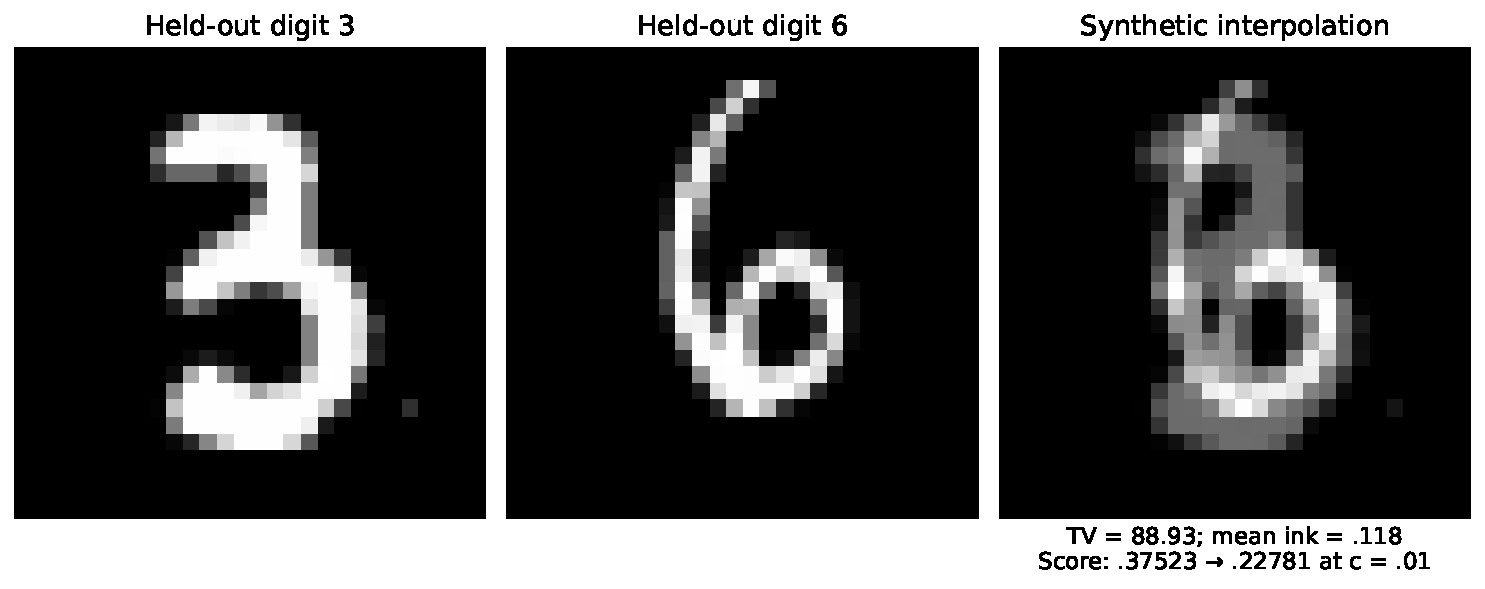
\includegraphics[width=.95\linewidth]{certificates/tv-boundary-counterexample.pdf}
\caption{An interpolation of opposite-parity held-out images, rounded to the eight-bit grid.  The interpolated image is synthetic and is not assigned a parity label.  At $c=.01$, a verified internal disturbance changes its clipped score by more than $.1474$, while every hidden state stays in $[-1,1]$.  Its TV and mean ink are within the stated smooth-image region.  This is a larger-radius example; the selected interpolation set passes numerical sufficient tests at $c=.001$ and $.003$.}
\label{fig:tv-boundary-counterexample}
\end{figure}

\section{Finite-radius certificates using reachable activation states}
\label{sec:reachable-tube}

A product of global operator norms ignores saturation. The following
certificate uses activation ranges reachable from one clean input under
\emph{all} disturbances in the prescribed ball. It applies at any radius;
small radii are not needed for its logical validity. The resulting bounds
can become conservative or vacuous at large radii.

Write the hidden network in column-vector notation as
$h_s=\tanh(a_s)$, $a_s=A_sh_{s-1}$, $1\le s\le H$, with a scalar readout
$z=v^\top h_H$. The input and its bias coordinate are fixed. Add
postactivation disturbances $\eta_s$ and output disturbance $\xi$, with
\[
 \sum_{s=1}^H\|\eta_s\|_2^2/N+\xi^2\le r^2.
\]
All clean activations, preactivations, and derivative matrices
$D_s=\operatorname{diag}(\operatorname{sech}^2a_s)$ below are fixed by this
input. Set $J_s=D_sA_s$ for $s\ge2$.

\paragraph{Forward enclosures.}
We construct a scalar $B_s$ and a nonnegative vector $C_s$ satisfying,
simultaneously for every allowed disturbance,
\[
 \|\Delta h_s\|_2\le B_s,\qquad |\Delta h_s|\le C_s.
\]
Initialize
$B_1=\sqrt N r$, $C_1=\sqrt N r\,\boldsymbol1$,
$q_1^{\rm lin}=q_1^{\rm tube}=1$, and $e_1=0$.
Given the preceding enclosures, set componentwise
\[
 b_{s,i}=\min\{\|(A_s)_{i,:}\|_2 B_{s-1},
                        (|A_s|C_{s-1})_i\}.
\]
Then the perturbed preactivation lies in
$[a_{s,i}-b_{s,i},a_{s,i}+b_{s,i}]$.
For the scalar remainder
\[
 R_a(u)=\tanh(a+u)-\tanh(a)-\operatorname{sech}^2(a)u,
\]
compute bounds $\rho^-_{s,i}\le R_{a_{s,i}}(u)\le\rho^+_{s,i}$ for
$|u|\le b_{s,i}$. Its exact extrema occur among the endpoints, $u=0$,
and $u=-2a_{s,i}$ when this point belongs to the interval: the derivative
vanishes exactly when $a+u=\pm a$. These extrema may be intersected with
any valid quadratic curvature bound. Put
$\rho_{s,i}=\max\{|\rho^-_{s,i}|,|\rho^+_{s,i}|\}$.

Choose upper bounds $\ell_s\ge\|J_s\|_{\rm op}$ and
\[
 L_s\ge\|U_sA_s\|_{\rm op},\qquad
 U_s=\operatorname{diag}\!\left(
  \operatorname{sech}^2((|a_{s,i}|-b_{s,i})_+)\right).
\]
Update
\begin{align*}
 q_s^{\rm lin}&=1+\ell_s^2q_{s-1}^{\rm lin},&
 e_s&=\ell_se_{s-1}+\|\rho_s\|_2,\\
 q_s^{\rm tube}&=1+L_s^2q_{s-1}^{\rm tube},&
 B_s&=\min\{\sqrt N r\sqrt{q_s^{\rm lin}}+e_s,
                    \sqrt N r\sqrt{q_s^{\rm tube}}\}.
\end{align*}
Finally set
\[
 C_{s,i}=\min\!\left\{B_s,\sqrt N r+
   \max_{u\in\{-b_{s,i},b_{s,i}\}}
          |\tanh(a_{s,i}+u)-h_{s,i}|\right\}.
\]
These intersections combine independent valid enclosures; they do not
assume that every disturbance can attain all their endpoints together.

\paragraph{Why the forward bounds hold.}
The exact perturbed recurrence is
$\Delta h_s=J_s\Delta h_{s-1}+\eta_s+R_s$, where $R_s$ lies in the
specified componentwise remainder interval. The sum of the clean linear
responses to all $\eta_j$ has norm at most
$\sqrt N r\sqrt{q_s^{\rm lin}}$, by Cauchy--Schwarz over the layerwise
noise norms and the products of the $\ell_j$. The propagated remainder
has norm at most $e_s$.
Independently, every mean-value derivative on the reachable interval has
coordinatewise absolute value bounded by $U_s$. Its operator norm is
therefore at most $\|U_sA_s\|_{\rm op}$: writing its diagonal derivative
as a diagonal contraction times $U_s$ proves this assertion.
Telescoping the nonlinear recurrence and using Cauchy--Schwarz now gives
$\sqrt N r\sqrt{q_s^{\rm tube}}$. The coordinate bound follows by
monotonicity of $\tanh$ and $|\eta_{s,i}|\le\sqrt N r$.
These arguments close the induction, including the use of the previously
intersected scalar and coordinate bounds to construct each new tube.

\paragraph{An output-specific interval.}
Define clean reverse adjoints
\[
 g_H=v,\qquad g_{s-1}=J_s^\top g_s,
 \qquad G=\sqrt{1+N\sum_{s=1}^H\|g_s\|_2^2}.
\]
Set $\rho_1^-=\rho_1^+=0$ and
\[
 E^- =\sum_{s,i}\min\{g_{s,i}\rho^-_{s,i},g_{s,i}\rho^+_{s,i}\},\qquad
 E^+ =\sum_{s,i}\max\{g_{s,i}\rho^-_{s,i},g_{s,i}\rho^+_{s,i}\}.
\]
Then every allowed disturbed output belongs to
\begin{equation}\label{eq:reachable-output-interval}
 [z-rG+E^-,\ z+rG+E^+].
\end{equation}
Indeed the exact output difference is
$\xi+\sum_sg_s^\top\eta_s+\sum_sg_s^\top R_s$.
The first two terms have absolute value at most $rG$; the last terms lie
between $E^-$ and $E^+$. One may further intersect this interval with
\[
 [z-T,z+T],\qquad
 T=r+\min\{\|v\|_2B_H,\ |v|^\top C_H\}.
\]
In particular these are finite-radius statements, not merely clean
Jacobian estimates.

For the clipped score $\psi_a(z)=\max\{-a,\min\{a,z\}\}$ and any verified
output interval $[l,u]$, the sufficient stability test is
\[
 \max\{|\psi_a(l)-\psi_a(z)|,|\psi_a(u)-\psi_a(z)|\}\le1/16.
\]
The main empirical convention uses $a=1/2$, with $a=1$ reported separately.
A saturated clean score may satisfy this test even when the raw output
interval is much wider than $1/8$. The certificate never requires a task
label or assumes that the clean prediction is correct.

Computing the clean adjoints costs $O(HN^2+Nd)$; computing all local
spectral norms costs $O(HN^3+Nd)$ for each input and radius. The construction
does not store the earlier $N$ by $HN$ transfer arrays. Our implementation
first tries cheaper global spectral bounds and reuses any certificate at
a larger radius for smaller radii. Ordinary float64 evaluations of these
real inequalities are reported as numerical sufficient tests; selected
claims receive separate interval or exact-rational verification. Checking
many data points or random cube points does not constitute a global
certificate. On a small finite cube, exhaustive coverage does.

\paragraph{A stronger refinement using signed clean transfers.}
When the preceding inexpensive bounds are inconclusive, one may retain
the full clean transfer matrices from all previous layers. Let $T_s$ map
RMS-normalized past disturbances to the current clean linear
preactivation response, so each injected hidden-noise block initially has
coefficient $\sqrt N I$. If all earlier nonlinear remainders have stacked
component bounds $\rho^-\le R\le\rho^+$, then each current preactivation
displacement lies in
\[
 \left[-r\|(T_s)_{i,:}\|_2+
  \frac{((T_s)_+\rho^-+(T_s)_-\rho^+)_i}{\sqrt N},\quad
  r\|(T_s)_{i,:}\|_2+
  \frac{((T_s)_+\rho^++(T_s)_-\rho^-)_i}{\sqrt N}\right].
\]
Here $(T_s)_+$ and $(T_s)_-$ denote its positive and negative parts.
The exact scalar remainder extrema above apply on this asymmetric
interval as well. Update the transfer matrix with the clean derivative
and append the new $\sqrt N I$ noise block. At the output use the same
signed interval propagation and include scalar output noise in the linear
Euclidean coefficient norm. This is an exact algebraic decomposition of
the perturbed recurrence, followed by interval bounds; no linearization
remainder has been discarded. It strengthens the earlier recurrence that
propagated only absolute remainder bounds. Its cost is $O(H^2N^3)$, so it
is used only where the cheaper certificates are inconclusive.

\paragraph{A verified saturated example.}
The preceding sufficient inequalities are mathematical statements; the large empirical tables evaluate them in ordinary float64 and are not themselves outward-rounded interval proofs.  We separately verified one illustrative finite-radius saturation certificate using outward intervals and exact integer-rational matrix bounds.  For the depth-32, width-128 MNIST 3-versus-8 SGD model used in the finite-grid counterexample, the fourth input in the fixed uniform held-out sample has clean output in a narrow interval around $8.282734267956$.  At $c=1/16$, reachable-tube derivative bounds prove
\[
 |z(x;\eta,\xi)-z(x;0,0)|<6.559413
\]
for every simultaneous hidden/output disturbance in the prescribed ball.  Consequently the clipped output is unchanged, for both cap $1/2$ and cap $1$.  This is a pointwise, all-disturbances certificate on one actual held-out image; it is not a claim about every input.  The same saved network has the verified finite-grid global counterexamples at $c=10^{-3}$ described above.  Thus the distinction between stability on data and global stability is present even in independently verified examples, and clipping can certify a useful condition when the raw-output variation bound is much larger than $1/16$.

For this computation, the clean trajectory is enclosed with 90-decimal outward interval arithmetic.  At each layer we round the reachable-tube upper derivative bounds upward to exact dyadic numbers.  For the resulting matrix $A=W\operatorname{diag}(D)$, the stored floating-point SVD merely proposes dyadic factors $U,S,V^T$.  All Gram matrices and the residual are recomputed with exact integers.  Writing
\[
 a=\|U^TU\|_\infty,\quad b=\|V^TV\|_\infty,
 \quad t=\max_i|S_{ii}|,\quad e^2=\|A-USV^T\|_F^2,
\]
we use the rational inequality
\[
 \|A\|_{\rm op}^2
 \le (1+\epsilon)t^2ab+(1+\epsilon^{-1})e^2,
 \qquad \epsilon>0.
\]
Here the matrix infinity norm is the maximum absolute row sum.  The bound follows from the symmetric Gram-matrix spectral bound, the triangle inequality, and Young's inequality, and makes no accuracy assumption about the proposed SVD.  Product rounding when constructing $A$ is enclosed by an additional exact Frobenius residual.  This yields a replayable certificate with saved dyadic factors.  It still trusts the interval library for transcendental evaluations and is not a Lean formalization.

\paragraph{A covariance refinement for a difficult vertex.}
Products of clean Jacobian norms can also be replaced by the exact covariance of the clean linear response.  In column-vector notation, write $J_s=D_sA_s$ for the clean hidden-state Jacobian, set $G_1=I$, and define
\[
 G_s=I+J_sG_{s-1}J_s^{\mathsf T}\qquad(s\ge2).
\]
If $T_s$ maps the stacked hidden disturbances to the clean linearized state, then $G_s=T_sT_s^{\mathsf T}$ by induction.  This is a deterministic Gramian identity; the certificate makes no Gaussian assumption about the disturbances.  Thus its linear part has norm at most $\sqrt N r\sqrt{\|G_s\|_{\rm op}}$.  Suppose coordinatewise Taylor remainder intervals on the already established preactivation tube imply a vector norm bound $R_s$.  With $\rho_1=0$, the recursion
\[
 \rho_s=\|J_s\|_{\rm op}\rho_{s-1}+R_s,
 \qquad
 B_s=\sqrt N r\sqrt{\|G_s\|_{\rm op}}+\rho_s
\]
then bounds the nonlinear remainder and total state displacement, respectively.  Indeed, subtracting the exact clean linear response gives $e_s=J_se_{s-1}+R_s(\Delta a_s)$, while each preactivation coordinate lies within $\|A_{s,j:}\|_2B_{s-1}$ of its clean value.  Finally,
\[
 |z^\eta-z|\le\|v\|_2B_H+r
\]
is a valid output bound, including the simultaneous scalar disturbance.  Using the full radius in both terms only makes this last bound conservative.

The implementation encloses each $G_s$ by outward-rounded dyadic interval matrix products.  An arbitrary dyadic midpoint proposal $M$ gives
$\|G_s\|_{\rm op}\le\|M\|_{\rm op}+\sup_{G\in[G_s]}\|G-M\|_F$;
both terms are bounded with exact rational matrix arithmetic and outward square roots.  Scalar remainder extrema occur at the two tube endpoints, zero, and $-2a$ when that critical point lies in the tube; intersecting this enclosure with $|R(u)|\le u^2/2$ is valid because $|\tanh''|\le1$.  No floating estimate of a covariance eigenvalue is accepted as a certificate.

\paragraph{Exact clean-output enclosures at dataset scale.}
For the finite held-out set, the stored float32 inputs and weights are
dyadic rational numbers. We approximate hidden states at denominator
$Q_h=2^{24}$ and weights at denominator $Q_w=2^{30}$, and compute all
approximate affine maps by integer matrix multiplication. Before every
product, an exact bound on the sum of absolute products rules out
signed 64-bit overflow, including intermediate accumulation.
The resulting affine arguments are therefore exact rational numbers.

The activation computation uses a piecewise-linear tanh table on
$[-12,12]$ with grid spacing $h=1/4096$. Every proposed table value is
independently enclosed using outward interval arithmetic. Since
$|\tanh''|\le1$, interpolation adds at most $h^2/8$ to the maximum
table-entry error; rounding the interpolated value adds at most
$1/(2Q_h)$. Outside the table, the approximation is the appropriate
sign and its error is at most $2e^{-24}$. Thus every approximate
activation has a common rigorously established coordinate error
$\tau$, without trusting floating-point evaluations of tanh.

If a clean hidden state is enclosed around its approximate value with
Euclidean error $e$, then the next state's error is at most
\[
 e'\le\|W\|_{\rm op}e
       +\sqrt N\,\|W-\widetilde W\|_F+\sqrt N\,\tau.
\]
Here $\|W\|_{\rm op}$ has an exact matrix-factor certificate,
the quantization residual is evaluated exactly, and the approximate
hidden coordinates remain in $[-1,1]$. The first layer separately
accounts for input quantization through the exact identity
\[
 xW-\widetilde x\widetilde W
  =x(W-\widetilde W)+(x-\widetilde x)\widetilde W.
\]
It uses column sums for the first term and exact integer products for
the second. The final scalar error is at most
$\|v\|_2e+\|v-\widetilde v\|_1$.
These bounds produce a clean-output interval at every recorded input.
Combining each interval with an independently verified global
disturbance bound gives a pointwise clipped-score certificate whenever
the resulting interval comparison succeeds. Every remaining input must
receive a separate local proof before a full held-out-set conclusion
is drawn. The method certifies the specified finite dataset, not the
input distribution or all possible images.

